\documentclass{beamer}[10pt, usepdftitle=false, handout]

\beamertemplatenavigationsymbolsempty

\usepackage[T1]{fontenc}
\usepackage[]{algorithm2e}
\usepackage{multimedia}
\usepackage{gensymb}
\usepackage{textcomp}

%\usepackage[font=small,labelfont=bf]{caption} 

\usetheme{Boadilla}

\title{Basic of Computer Networks 5}
\author[]{Paul Blondel}
\institute[]{CNAM}
\date[]{March 1st, 2019}

\usepackage[style=british]{csquotes}


\def\signed #1{{\leavevmode\unskip\nobreak\hfil\penalty50\hskip1em
  \hbox{}\nobreak\hfill #1%
  \parfillskip=0pt \finalhyphendemerits=0 \endgraf}}

\newsavebox\mybox
\newenvironment{aquote}[1]
  {\savebox\mybox{#1}\begin{quote}\openautoquote\hspace*{-.7ex}}
  {\unskip\closeautoquote\vspace*{1mm}\signed{\usebox\mybox}\end{quote}}


\setbeamertemplate{headline}
{
  \leavevmode%
  \hbox{%
  \begin{beamercolorbox}[wd=1.0\paperwidth,ht=2.25ex,dp=1ex,center]{author in head/foot}%
    \usebeamerfont{author in head/foot}\insertsubsection
  \end{beamercolorbox}}%
  \vskip0pt%
}


\setbeamertemplate{footline}
{
  \leavevmode%
  \hbox{%
  \begin{beamercolorbox}[wd=.5\paperwidth,ht=2.25ex,dp=1ex,center]{author in head/foot}%
    \usebeamerfont{author in head/foot}\insertsection
  \end{beamercolorbox}%
  \begin{beamercolorbox}[wd=.5\paperwidth,ht=2.25ex,dp=1ex,center]{title in head/foot}%
    \usebeamerfont{title in head/foot} \inserttitle \hspace*{2em}  \insertframenumber{} / \inserttotalframenumber\hspace*{2ex} 
  \end{beamercolorbox}}%
  \vskip0pt%
}

\AtBeginSection[]
{
   \begin{frame}
    \tableofcontents[ 
    currentsection] 
   \end{frame}
}

\begin{document}
	{
	\setbeamertemplate{footline}{
  	\leavevmode%
  	\hbox{%
  	\begin{beamercolorbox}[wd=.5\paperwidth,ht=2.25ex,dp=1ex,center]{author in head/foot}%
  	\end{beamercolorbox}%
  	\begin{beamercolorbox}[wd=.5\paperwidth,ht=2.25ex,dp=1ex,center]{title in head/foot}%
  	\end{beamercolorbox}}%
  	\vskip0pt%	
	} 
	\begin{frame}
	\titlepage
	\end{frame}

	\begin{frame}
	
	\begin{aquote}{Tim-Bernes Lee - Creator of the WEB}
I think, in general, it's clear that most bad things come from misunderstanding, and communication is generally the way to resolve misunderstandings — and the Web's a form of communications — so it generally should be good.
	\end{aquote}	
	
	\end{frame}


	\begin{frame}
		\tableofcontents
	\end{frame}
	}

	\addtocounter{framenumber}{-3}

	\section{Local Area Networks}
	\subsection{Introduction}

    \begin{frame}[label=(first)]
		
	What is a Local Area Network (or LAN)?
	\vspace*{1em}
	
	\begin{itemize}
	\item{A local area network is a communication network that interconnects a variety of data communicating devices within a small geographic area and broadcasts data at high data transfer rates with very low error rates}
	
	\item{Since the local area network first appeared in the 70s, its use has become widespread in commercial and academic environments.}
	\item{Actually nowadays everybody has a LAN at home (the internet Box)}
	\end{itemize}

		\begin{center}	
	\begin{figure}
		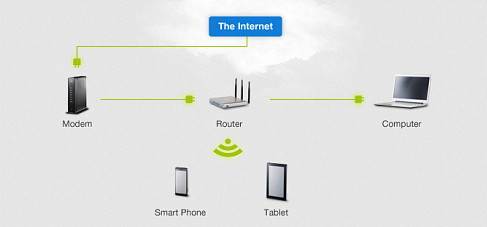
\includegraphics[scale=0.4]{images/5-1.png} 
     	%\vspace*{-0.5em}
		%\caption{Floating gate transistor cell}
	\end{figure}	
	\end{center}

	
	\end{frame}

	
	\subsection{Advantages of LANs}
	
	\begin{frame}
	
	Advantages of LANs:
	\vspace*{1em}	
	
	\begin{itemize}
	\item{Ability to share hardware and software resources.}
	\item{Local computers can survive internet failure and still exchange information each other.}
	\item{Computers of the LAN can exchange information at high speed and independently (no need MAN/WAN accesses).}	
	\item{Private ownership: only the computers belonging to the LAN can access the shared information (if not connected to Internet or properly secured from other networks)}
	\item{The error rate is generally much less important.}
	\end{itemize}		
			
	
	\end{frame}	
	
	\subsection{Disadvantages of LANs}	
	
	\begin{frame}
	
	Disadvantages of LANs:
	\vspace*{1em}	
	
	\begin{itemize}
	
	\item{You can only access geographically close computers...}
	\item{Designing a LAN can sometimes be difficult and costly (especially in industrial environments).}
	\item{Some types of hardware may not inter-operate easily.}
	\item{A LAN is only as fast as its slowest link!}	
	
	\end{itemize}		
		
	\end{frame}	
	
	\section{LAN Topologies}
		
	\begin{frame}
	
	Most Local Area Networks are based on one of these three main topologies:
	\vspace*{1em}	
	
	\begin{enumerate}
	\item{The Bus Topology}
	\item{The Star Topology}
	\item{The Ring Topology}
	\end{enumerate}		
	
	\end{frame}		
		
	\subsection{Bus Topology}		
		
	\begin{frame}
	
	The Bus	Topology:
	\vspace*{1em}
	
	\begin{itemize}
	\item{Shared medium main interconnect}
	\item{Each computer has a connection to the medium}
	\end{itemize}		
	
	\begin{center}	
	\begin{figure}
		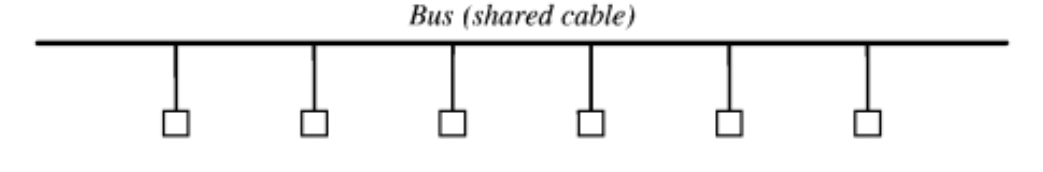
\includegraphics[scale=0.4]{images/5-4.png} 
     	%\vspace*{-0.5em}
		%\caption{Floating gate transistor cell}
	\end{figure}	
	\end{center}	
	
	\begin{block}{Note}
	\begin{itemize}
	\item{Easy to add a node to the network (without disturbing the network)}
	\item{Resilient to computer failure(s)}
	\item{Data transmission management is complex}
	\end{itemize}
	\end{block}
			
	\end{frame}			
		
		
	\subsection{Star Topology}
	
	\begin{frame}
	
	The Star Topology:
	\vspace*{1em}	
	\begin{itemize}
	\item{The central component of the network is known as hub or switch}
	\item{Each computer has a separate connection to the hub}
	\end{itemize}		
	
	\begin{center}	
	\begin{figure}
		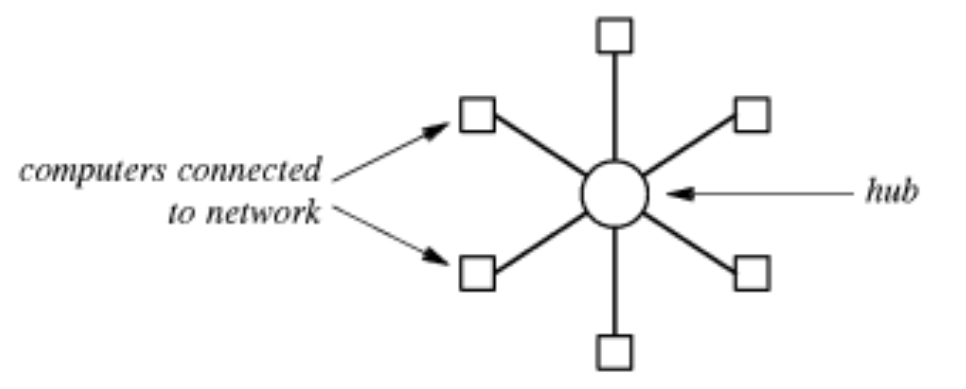
\includegraphics[scale=0.3]{images/5-2.png} 
     	%\vspace*{-0.5em}
		%\caption{Floating gate transistor cell}
	\end{figure}	
	\end{center}
	
	\begin{block}{Notes}
	\begin{itemize}
	\item{If a node (=computer) of the network is disconnected the network still works}
	\item{Node to node exchanges are optimized (information simply transit through the switch)}
	\end{itemize}
	\end{block}
		
	
	\end{frame}			

	\subsection{Ring Topology}
	
	\begin{frame}
	
	The Ring Topology:
	\vspace*{1em}
		
	\begin{itemize}
	\item{No central facility (no switch needed)}
	\item{Connections go directly from one computer to another}
	\item{Invented by IBM in the 80s}
	\end{itemize}
	
	\begin{center}	
	\begin{figure}
		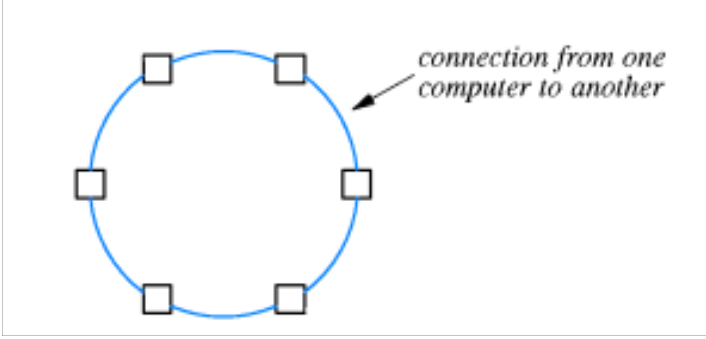
\includegraphics[scale=0.3]{images/5-3.png} 
     	%\vspace*{-0.5em}
		%\caption{Floating gate transistor cell}
	\end{figure}	
	\end{center}
	
	\begin{block}{Notes}
	\begin{itemize}
	\item{If one node (=computer) does not work: the ring network is cut!}
	\item{Data transmission management can be simplified with this topology}	
		
	\end{itemize}	
	\end{block}	
	
	
	\end{frame}		
		
	\section{Bus Network}
	
	\begin{frame}
	
	Before talking about Bus Network, let's talk about Ethernet:
	\vspace*{1em}
	
	Ethernet ...
	\vspace*{1em}
	
	\begin{itemize}
	\item{... is a computer network technology}
	\item{... is the most popular wired LAN technology}
	\item{... can have different wiring schemes}
	\item{... can have different data rates (nowadays: up to the gigabyte/sec}
	\item{... is the fruit of the IEEE 802.3 standard}
	\end{itemize}		

	\begin{center}	
	\begin{figure}
		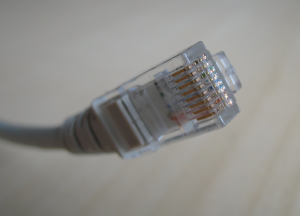
\includegraphics[scale=0.3]{images/5-5.png} 
     	%\vspace*{-0.5em}
		%\caption{Floating gate transistor cell}
	\end{figure}	
	\end{center}
	
	
	You all know this famous RJ45 Ethernet cable ...
	
	\end{frame}	
	
	\begin{frame}
	
	\begin{center}	
	\begin{figure}
		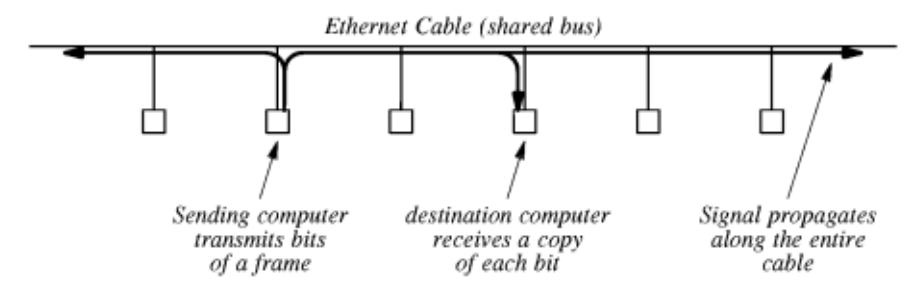
\includegraphics[scale=0.4]{images/5-6.png} 
     	%\vspace*{-0.5em}
		%\caption{Floating gate transistor cell}
	\end{figure}	
	\end{center}
		
	In this case:
	\vspace*{1em}
	\begin{itemize}
	\item{Nodes transmit data using a same shared medium.}
	\item{Signal propagates across the entire cable.}
	\item{All nodes receive the data.}
	\item{Collisions of information may occur! The solution is CSMA/CD.}
	\end{itemize}
		
	\end{frame}		
	
	\subsection{The CSMA/CD Pradigm}
	\begin{frame}
	
	Some collisions may occur with the Bus Topology, example:
	\vspace*{1em}

	\begin{center}	
	\begin{figure}
		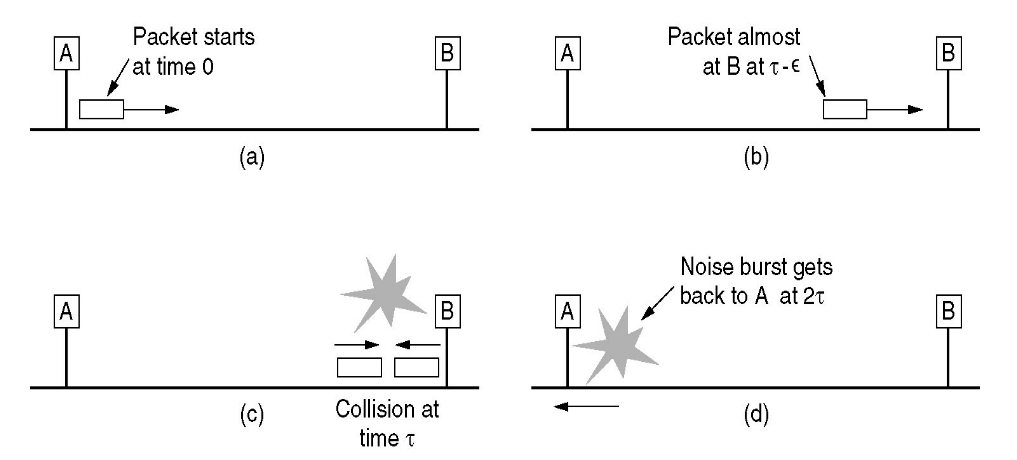
\includegraphics[scale=0.4]{images/5-7.png} 
     	%\vspace*{-0.5em}
		%\caption{Floating gate transistor cell}
	\end{figure}	
	\end{center}


	\begin{block}{Notes}
	\begin{itemize}
	\item{Collision detection can take as long as 2 times one-way propagation delay in worst case!}
	\item{The CSMA/CD Paradigm is an approach to handle these cases.}
	\end{itemize}
	\end{block}
		
	\end{frame}	
	
	\begin{frame}
	
	But what is the CSMA/CD Paradigm?	
	\vspace*{1em}
	
	\begin{itemize}
	\item{MA: Multiple Access
		\begin{itemize}
			\item{Multiple computers are attached to a shared medium}
			\item{Each uses a same access algorithm}	
		\end{itemize}
	}
	\item{CS: Carrier Sense
		\begin{itemize}
		\item{Wait until the medium is free}
		\item{Then transmit the frame}
		\end{itemize}
	}
	\item{CD: Collision Detection}
	\item{With CSMA/CD: simultaneous transmissions are possible!}	
	\end{itemize}
		
	\end{frame}	
	
	
	\begin{frame}
	
	How does it work?	
	\vspace*{1em}
	
	When two transmissions interfere with one another we have a collision.
	\vspace*{0.5em}
	
	With the CSMA/CD Paradigm the node ... 
	\begin{itemize}
	\item{... listens to the medium during transmission}
	\item{... detects whether another node's signal interferes
	\begin{itemize}
		\item{If the emitting node receives another signal during the transmission of its signal, it means there is a collision}
	\end{itemize}
	}
	\item{... transmits again the signal in case of collision detection (back off)}
	\end{itemize}		
		
	\end{frame}
	
	\begin{frame}
	
	When do we decide to re-transmit the signal with the CSMA/CD Paradigm?
	\vspace*{1em}

	\begin{itemize}
	\item{When a collision occurs: it waits a random time $t_1$ ($0\leq t_1 \leq d$)}
	\item{If a second collision occurs afterwards: it waits a random time $t_2$ ($0\leq t_2\leq 2\times d$)}	
	\item{For each successive collision: the range is doubled.}
	\item{It is called: exponential backoff}
	\end{itemize}
	
	\end{frame}	
	
	\section{Ring Network}
	
	\begin{frame}
	
	The Ring Network:
	\vspace*{1em}	
	
	\begin{itemize}
	\item{Once a popular topology for LANs}
	\item{Bits flow in single direction}
	\end{itemize}
	
	\begin{center}	
	\begin{figure}
		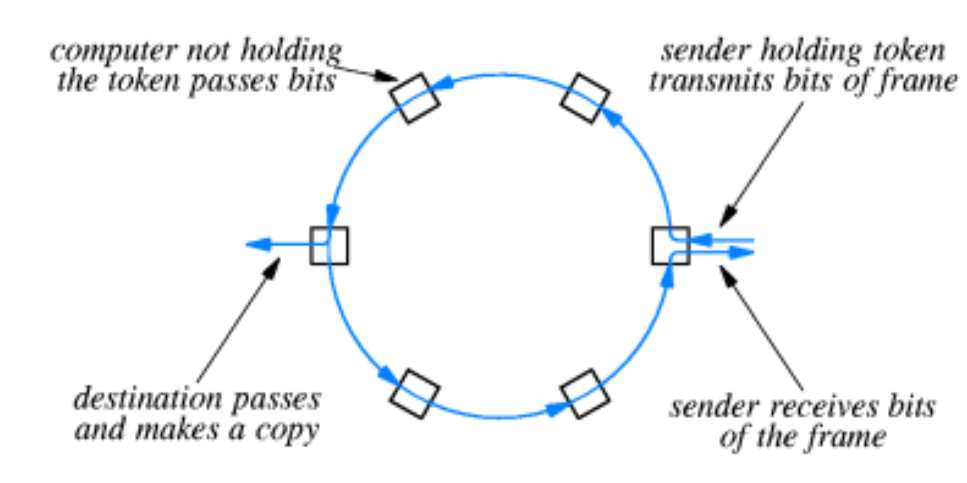
\includegraphics[scale=0.3]{images/5-10.png} 
     	%\vspace*{-0.5em}
		%\caption{Floating gate transistor cell}
	\end{figure}	
	\end{center}
	
	\begin{block}{Note}
	A token is transmitted from one node to node. The node having the token can transmit the data.
	\end{block}	
		
	\end{frame}		
	
	\subsection{Token Passing Paradigm}	
		
	\begin{frame}
	
	The token passing paradigm:
	\vspace*{1em}
	\begin{itemize}
	\item{It is designed for ring topology}
	\item{It guarantees fair access}
	\item{Token:
		\begin{itemize}
			\item{It is a special message (reserved)}
			\item{It's just small (a few bits)}
		\end{itemize}
	}
	\end{itemize}		
		
	\end{frame}
	
	\begin{frame}
	
	How it works:
	\vspace*{1em}
		
	\begin{itemize}
	\item{Each node:
		\begin{itemize}
			\item{waits for token to arrive}
			\item{transmits one packet around ring}
			\item{transmits token around ring}
		\end{itemize}			
	}
	\item{When no node has data to send
		\begin{itemize}
			\item{token circulates continuously}
		\end{itemize}			
	}	
	\end{itemize}		
		
	
	\end{frame}	
	
	\begin{frame}
	
	Token ring topology pros and cons:
	\vspace*{1em}	

	Pros:
	\vspace*{0.5em}		
	
	\begin{itemize}
	\item{Intermediate hardware (switch or hub) not needed}
	\item{A better management of packet transmission (no need of CSMA/CD or CSMA/CA)}
	\end{itemize}
	
	Cons
	\vspace*{0.5em}	
				
	\begin{itemize}
	\item{A broken wire disables the ring!}
	\item{Difficult to add/move/remove node with this topology.}
	\end{itemize}
				
	
	\end{frame}	
	
	
	\begin{frame}
	
	Some token ring approaches use two rings (one inner ring and one outer ring) to be resilient in case one node is malfunctioning:
	\vspace*{1em}	
			
				
	\begin{center}	
	\begin{figure}
		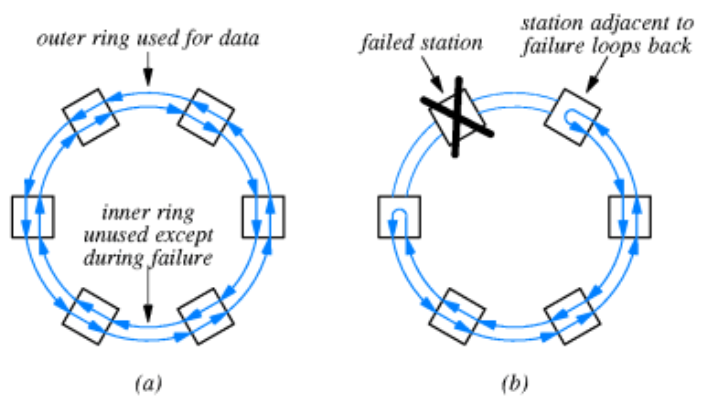
\includegraphics[scale=0.4]{images/5-11.png} 
     	%\vspace*{-0.5em}
		%\caption{Floating gate transistor cell}
	\end{figure}	
	\end{center}	
			
	\begin{itemize}
	\item{When working normally one ring is used}
	\item{Second ring is used for loopback during failure}
	\end{itemize}
	
	\begin{block}{Note}
	Only one node can fail with this approach!
	\end{block}	
	
	
	\end{frame}	
	
	
	
	\section{Wireless LAN}	
	
	
	\begin{frame}
	
	With wireless LANs ...
	\vspace*{1em}
	
	\begin{itemize}
	\item{... not all nodes receive all transmissions}
	\item{... cannot use CSMA/CD in this case! Not useful.}
	\end{itemize}		

		\begin{center}	
	\begin{figure}
		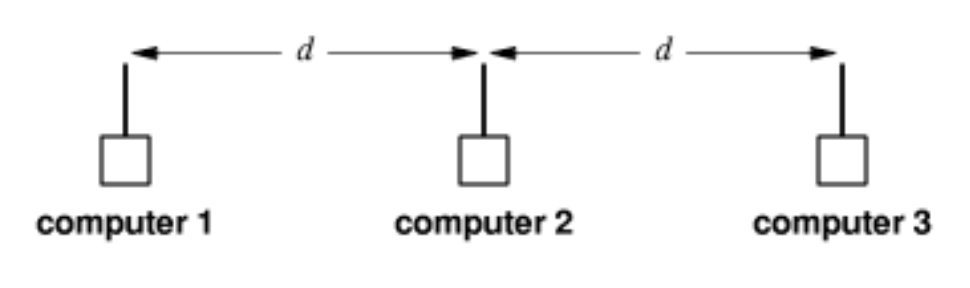
\includegraphics[scale=0.3]{images/5-8.png} 
     	%\vspace*{-0.5em}
		%\caption{Floating gate transistor cell}
	\end{figure}	
	\end{center}


	\begin{block}{Notes}
	\begin{itemize}
	\item{Maximum transmission distance is $d$.}
	\item{Nodes 1 and 3 do not receive each other' transmissions.}
	\end{itemize}	
	\end{block}

	\end{frame}	
		
	\begin{frame}
	
	Hidden and Exposed Terminal Effects:
	\vspace*{1em}
	
	\begin{center}	
	\begin{figure}
		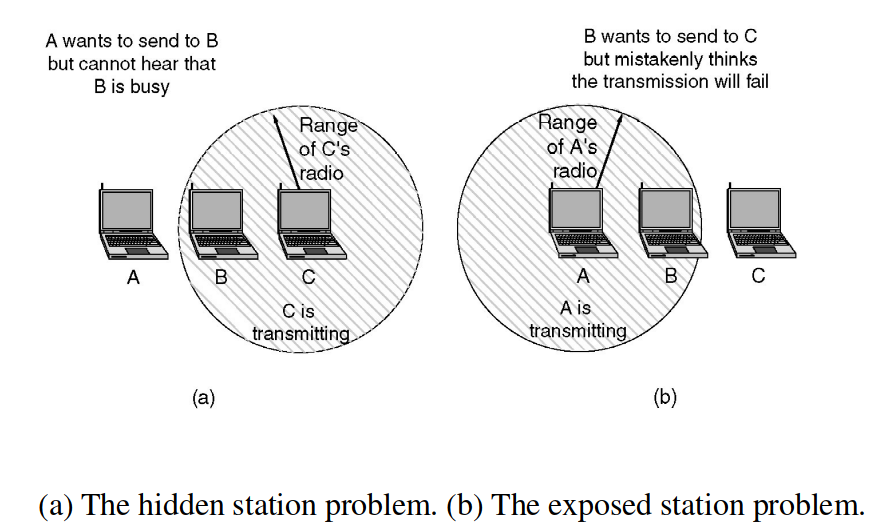
\includegraphics[scale=0.4]{images/5-9.png} 
     	%\vspace*{-0.5em}
		%\caption{Floating gate transistor cell}
	\end{figure}	
	\end{center}
	
	\begin{block}{Note}
	A solution to this is the CSMA/CA Paradigm!
	\end{block}	
	
	\end{frame}		

	\subsection{The CSMA/CA Paradigm}
	
	\begin{frame}
	
	The CSMA/CA Paradigm:
	\vspace*{1em}	
	
	The CSMA/CA Paradigm is based on collision avoidance (and not detection!).
	\vspace*{0.5em}
			
	\begin{itemize}
	\item{Used on wireless LANs!}	
	\item{Both sides send small messages before the data transmission itself!
		\begin{itemize}
		\item{"X is about to send to Y": Give me some place!!}
		\item{"Y is about to receive from X": Don't send me things!!}
		\item{Data frame is finally sent from X to Y}
		\end{itemize}
	}
	\item{The purpose is to inform all nodes in range of X or Y before transmission.}
	\item{CA: Collission Avoidance}
	\end{itemize}		
		
	\end{frame}	

	\section{Summary}
	
	\begin{frame}
	
	\begin{itemize}
	\item{LANs are designed for short distance data exchanges}
	\item{Three main topologies: Bus, Ring and Star.}
	\item{The most popular LAN technology is Ethernet}
	\item{Apart from that, wireless LANs are also very popular}
	\item{Although interesting the Token Ring approach is less popular}
	\end{itemize}		
		
	\end{frame}	
	
		
	
\end{document}